\documentclass[12pt,a4paper]{report}
\usepackage[utf8]{inputenc}
\usepackage[T1]{fontenc}
\usepackage[francais]{babel}
\usepackage[colorlinks=true]{hyperref}
\usepackage{graphicx}
\hypersetup{urlcolor=blue,linkcolor=black,citecolor=black,colorlinks=true}

\newcommand{\myTitle}{
\begingroup 
\centering 


\vspace{\stretch{1}}
{\LARGE Le support des r\'{e}seaux mobiles dans IPv6}% Title

\vspace*{1\baselineskip}

\LARGE % Small caps
Le protocole NEMO
\vspace{\stretch{2}}

\vspace{\stretch{1}}
{\Large SARI Soumia \& Kaoutar Sarah SANFILIPPO\par} 
\vspace{\stretch{2}}

\vspace{\stretch{1}}
{\large 2014 - 2015}
\vspace{\stretch{2}}%pour gérer les espaces sur des pages,  \stretch{} fait des espaces proportionnels
\setcounter{page}{0}

\endgroup}


\begin{document}
\thispagestyle{empty}
\myTitle

\renewcommand{\contentsname}{Sommaire}
\tableofcontents

\newpage
\section{Introduction}

L'explosion des technologies de communication sans fil (e.g. Wi-Fi) a fait \'{e}merger un nouveau
concept dans les r\'{e}seaux IP : la mobilit\'{e}. Lorsqu'un utilisateur b\'{e}n\'{e}ficie d'une connexion sans fil \`a
l'Internet, celui-ci peut se d\'{e}placer tout en communiquant. Cependant, de tels d\'{e}placements
requi\'{e}rent un support sp\'{e}cifique au niveau de la couche 3 du mod\`{e}le TCP/IP, sans lequel toutes les
communications seront rompues lors d'un changement de sous-r\'{e}seaux IPv6. Pour palier ces
probl\`{e}mes, l'organisme de standardisation IETF a d\'{e}fini le protocole NEMO (Network Mobility) Basic
Support qui place la gestion de la mobilit\'{e} au niveau des routeurs, ce qui permet le mouvement de
r\'{e}seaux entiers tout en conservant la complexit\'{e} de la gestion des d\'{e}placements dans l'Internet sur
ces dits routeurs.\cite{ref}

\section{Historique}

Le groupe NEMO de l'IETF a fait son apparition en octobre 2002 , et a standardiser une solution simple connu sous
le nom de NEMO BASIC SUPPORT d\'eriv\'e de Mobile IP pour g\'er\'e la mobilit\'e des r\'eseaux.
Un des objectifs est de ne pas imposer des modifications aux noeuds mobiles.
 
\section{R\'eseaux NEMO}
Un r\'eseau mobile ou r\'eseau NEMO peut \^etre d\'efini comme un r\'eseau /sous-r\'eseau en d\'eplacement, connect\'e \`a Internet par l'interm\'ediaire d'un ou plusieurs routeurs qui changent leurs points d'attachements dans la topologie Internet. La gestion de la mobilit\'e des r\'eseaux NEMO doit assurer d'une mani\`ere transparente la continuit\'e des services Internet  pour les stations ou terminaux embarqu\'e.

\section{Protocol Nemo  Basic Support (BS)}
Le protocole NEMO BS est une extension de MIPV6 pour supporter la mobilit\'{e} d'un 
r\'{e}seau entier (r\'{e}seau NEMO) qui change son point d'attachement \`{a} Internet. NEMO BS  assure d'une mani\`ere transparente la continuit\'e des sessions ouvertes pour tous les nœuds dans le r\'eseau mobile NEMO.

\newpage
\section{Fonctionnement  de base du protocole NEMO BS}

Gr\^ace \`a l'introduction d'un routeur appel\'e routeur mobile (Mobile Router, MR) qui est l'entit\'e la plus importante  au niveau du r\'eseau NEMO.
 Le réseau NEMO est attach\'e au r\'eseau m\`ere/r\'eseau visit\'e par le biais du routeur mobile (MR) qui contr\^ole son mouvement. 
Toutes les communications depuis et vers les nœuds mobiles (Mobile Network Nodes, MNN) situés au sein du r\'eseau NEMO passent \`a travers le MR, le changement de point d'acc\`es ne provoque pas de changement d'adresse IP de MNN.
Un pr\'efixe IPv6 (Mobile Network Prefix, MNP) est d\'el\'egu\'e par le Home Agent (HA) au MR pour l’annoncer aux MNNs situ\'es au sein du r\'eseau NEMO.
Le MR admet au minimum deux interfaces : une interface interne (Ingress Interface,  IIF) et une interface externe (Egress Interface,  EIF). L'interface IIF est configur\'ee avec une adresse IP prise du pr\'efixe MNP, tandis que l'interface EIF est configur\'ee avec l'adresse HoA lorsque le r\'eseau NEMO (plus pr\'ecis\'ement le MR) est attach\'e au r\'eseau m\`ere (Home Network), c'est l'adresse m\`ere unique par laquelle il est accessible quand il est li\'e au r\'eseau m\`ere. Lorsque le MR est attach\'e \`a un r\'eseau visit\'e, l'interface EIF sera configur\'ee avec une adresse temporaire CoA \cite{benaouda2014etude}

\begin{figure}[h]
\begin{center}
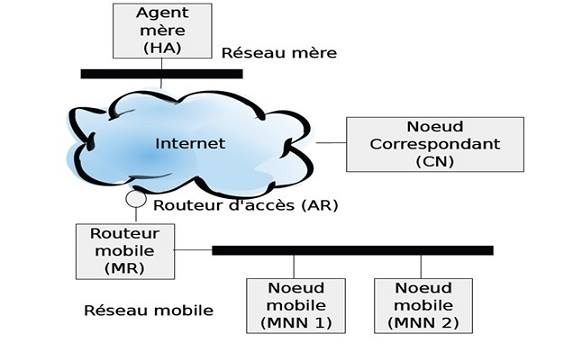
\includegraphics[scale=0.7]{img8.png}
\caption[9pt]{Fig.1 Architecture}
\end{center}
\end{figure}

\newpage
\section{Sc\'{e}nario}

Apr\`{e}s avoir d\'{e}marr\'{e}, le routeur mobile se configure automatiquement pour assurer une connectivit\'{e} aux utilisateurs associ\'{e}s. Ces derniers vont pouvoir automatiquement d\'{e}couvrir des services IPv6 fournis par l'op\'{e}rateur. Enfin, le routeur en mouvement passant d'un r\'{e}seau d'acc\`{e}s à un autre conserve les connexions r\'{e}seaux de mani\`{e}re transparente pour l'utilisateur.
\begin{figure}[h]
\begin{center}
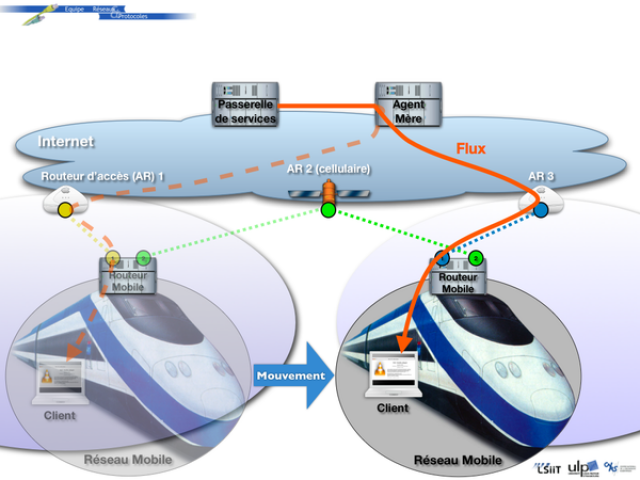
\includegraphics[scale=0.7]{R2.png}
\caption[9pt]{Fig.2 Exemple de r\'{e}seau mobile embarquant un routeur mobile munis de multiples interfaces. Le routeur mobile assure la continuit\'{e} de service tout au long des d\'{e}placements du train.}
\end{center}
\end{figure}

\newpage
\paragraph{Gestion de la Mobilit\'{e}:} 
Le routeur mobile op\`{e}re le protocole NEMO BS qui lui permet d'\^{e}tre toujours joignable par l'interm\'{e}diaire de son adresse principale tout comme les clients associ\'{e}s dans le r\'{e}seau mobile. Cette adresse principale est associ\'{e}e \'{a} une adresse temporaire aupr\`{e}s d'un \'{e}quipement appel\'{e} agent m\`{e}re. Cette adresse temporaire repr\'{e}sente la position r\'{e}elle du routeur mobile dans la topologie d'Internet et est mise-\'{a}-jour \'{a} chaque d\'{e}placement du r\'{e}seau mobile vers un nouveau r\'{e}seau d'acc\'{e}s.
L'ensemble des flux \'{a} destination du r\'{e}seau mobile passent toujours par l'agent m\`{e}re, qui peut donc assurer la continuit\'{e} des flux tout au long des d\'{e}placements du r\'{e}seau mobile.

\paragraph{Multi-domiciliation:} 
Le routeur mobile dispose de plusieurs interface r\'{e}seau lui permettant de se connecter en parall\`{e}le a plusieurs r\'{e}seaux d'acc\`{e}s IPv6. Son adresse principale est alors associ\'{e}e \`{a} plusieurs adresses IPv6 temporaires (une par interface) gr\^{a}ce au protocole Multiple Care-of Addresses registration (MCoA). Plusieurs chemins concurrents peuvent ainsi \^{e}tre maintenus entre le routeur mobile et son agent m\`{e}re.
Les flux de l'Internet \'{a} destination du r\'{e}seau mobile ou inversement font l'objet d'une d\'{e}cision de routage respectivement sur l'agent m\`{e}re ou le routeur mobile. Ces d\'{e}cisions sont prises en fonction de \'{e}\'{e}rences ou politiques de routages pr\'{e}sentes sur chacune de ces entit\'{e}s.
Les flux peuvent ainsi \^{e}tre partag\'{e}s entre diff\'{e}rent chemins selon leur protocol et/ou port. Le routeur mobile et l'agent m\`{e}re peuvent \'{e}galement plus facilement faire face \'{a} une panne ou une d\'{e}connexion de l'un des r\'{e}seaux d'acc\`{e}s en redirigeant les flux vers les interfaces disponibles.
Nous travaillons \'{e}galement \'{a} la gestion de routeurs mobiles multiples au sein d'un m\^{e}me r\'{e}seau mobile. Nous nous int\'{e}ressons notamment aux m\'{e}canismes de redondance des routeurs mobiles tout en \'{e}tendant la mise en oeuvre du partage de charge et de tol\'{e}rance au fautes dans ce contexte. \cite{ref3}

\newpage
\section{Contraintes}
La gestion de la mobilit\'e des r\'eseaux mobiles doit se faire face \`a de nombreuse contraintes:
\begin{enumerate}
  \item il convient de supporter les r\'eseaux mobiles en nombre et en taille importantes , en consid\'erant divers types de configuration ( un seul sous-r\'eseau , la multi-domiciliation, la mobilit\'e enchain\'ee).
  \item Le nombre \'elev\'e de correspondants nous impose de minimiser la quantit\'e de messages de controle relatifs \`a la gestion de la mobilit\'e tout en optimisant le routage.
  \item Ces messages doivent \^etre \'echang\'es en toute s\'ecurit\'e et authentifi\'es par leurs destinataires pour s'assur\'er qu'ils ne sont pas envoy\'es par un usurpateur. \cite{referance}
\end{enumerate}

\section{Conclusion}
Le support des r\'eseaux mobiles est \`a pr\'esent un sujet qui int\'eresse se nombreux industriels, allant des fournisseurs
 d'\'equipement r\'eseaux ou d'\'electronique grand publique jusq'aux fabriquant d'automobiles, en passant par les op\'erateurs de t\'elephone et de transport public. 

\bibliographystyle{unsrt} %plain, unsrt, alpha, abbrv, acm, apalike
\bibliography{nemo} % mon fichier de base de données s'appelle bibli.bib

\end{document} 
